\documentclass[../notes.tex]{subfiles}

\pagestyle{main}
\renewcommand{\chaptermark}[1]{\markboth{\chaptername\ \thechapter\ (#1)}{}}
\setcounter{chapter}{7}

\begin{document}




\chapter{Electronic Structure of Atoms and Molecules}
\section{Hybridization and Time-Dependent Quantum Mechanics}
\begin{itemize}
    \item \marginnote{11/15:}Consider \ce{BeH2}.
    \begin{itemize}
        \item Then we can form the $sp$ molecular orbital
        \begin{equation*}
            \psi_{sp} = \frac{1}{\sqrt{2}}(2s\pm 2p_z)
        \end{equation*}
        \item Draws an orbital diagram of \ce{BeH2}.
    \end{itemize}
    \item \ce{BH3}.
    \begin{itemize}
        \item Lists $sp^2$ hybrid orbital wave functions.
    \end{itemize}
    \item \ce{CH4}.
    \begin{itemize}
        \item Lists $sp^3$ hybrid orbital wave functions.
    \end{itemize}
    \item The probability of finding a $\psi_1$ electron in the $2p_z$ orbital.
    \begin{itemize}
        \item The absolute value of the coefficient of $2p_z$ in the wave function, squared.
        \item Alternatively,
        \begin{equation*}
            \Prob = \left| \int 2p_z^*\psi_1\dd{\tau} \right|^2
        \end{equation*}
    \end{itemize}
    \item Time-dependent Schr\"{o}dinger equation:
    \begin{equation*}
        \hat{H}\psi = i\hbar\dv{\psi}{t}
    \end{equation*}
    \begin{itemize}
        \item Let $\psi_n(r,t)=\phi_n(r)\e[-iE_nt/\hbar]$. Plugging this into the time-dependent Schr\"{o}dinger equation yields
        \begin{align*}
            \hat{H}\psi &= i\hbar\dv{t}(\phi_n(r)\e[-iE_nt/\hbar])\\
            &= i\hbar\cdot-\frac{iE_n}{\hbar}\cdot\phi_n(r)\e[-iE_nt/\hbar]\\
            &= E_n\psi_n
        \end{align*}
        \item Thus, to this point, we've been solving the spatial part of the time-dependent Schr\"{o}dinger equation.
        \item The probability density of the time-dependent solution is equal to the probability density of the time-independent solution.
        \begin{align*}
            |\psi(r,t)|^2 &= \left| \phi(r)\e[-iEt/\hbar] \right|^2\\
            &= \psi^*(r)\psi(r)\e[iEt/\hbar]\e[-iEt/\hbar]\\
            &= \psi^*(r)\psi(r)\\
            &= |\psi(r)|^2
        \end{align*}
    \end{itemize}
    \item The time-dependent Schr\"{o}dinger equation allows us to make predictions for how long it takes an electron to relax back to a lower energy state after excitation, for instance.
    \item Using the time-dependent Schr\"{o}dinger equation to describe the interaction of the system with electromagnetic radiation.
    \begin{enumerate}
        \item Solution: $\vec{E}=\vec{E}_0\cos(\omega t)$\footnote{This is the definition of a classical electric radiation field. In Advanced Quantum Mechanics, we can turn this into a photon field for quantum electrodynamics.}.
        \item Dipole moment of the molecule ($\mu$).
    \end{enumerate}
    \begin{itemize}
        \item We let $\hat{V}=-\vec{\mu}\cdot\vec{E}$. This is how radiation interacts with matter.
        \item This leads to the overall Hamiltonian for the molecule interacting with the electric field as $\hat{H}=\hat{H}_0+\hat{V}$, where $\hat{H}_0$ is the Hamiltonian of the molecule and $\hat{V}$ is the dipole-electric field perturbation defined above.
        \item If the electron is transitioning from the ground to the first-excited state, we let
        \begin{equation*}
            \psi(t) = a_1(t)\phi_1\e[-iE_1t/\hbar]+a_2(t)\phi_2\e[-iE_2t/\hbar]
        \end{equation*}
        where the first part refers to the ground state, the second part refers to the excited state, and $a_1,a_2$ are time-dependent expansion coefficients that we are solving for.
        \item Substitution into the time-dependent Schr\"{o}dinger equation yields
        \begin{align*}
            i\hbar\left( \psi_1\dv{a_1}{t}+\psi_2\dv{a_2}{t} \right) &= a_1(t)\hat{V}\psi_1+a_2(t)\hat{V}\psi_2\\
            i\hbar\e[-iE_2t/\hbar]\dv{a_2}{t} &= a_1(t)\int\phi_2^*\hat{V}\psi_1\dd{\vec{r}}+a_2(t)\int\phi_2^*\hat{V}\psi_2\dd{\vec{r}}
        \end{align*}
    \end{itemize}
\end{itemize}



\section{Time-Dependent Schr\"{o}dinger Equation}
\begin{itemize}
    \item \marginnote{11/17:}The TD SE is an \textbf{initial value differential equation} since we know $\psi_0$ and can propagate that over time.
    \item We will approximate the solutions to this with both an expansion (variational method) and perturbation theory.
    \item Now we continue from before (finding the time-dependence of the interaction of a EM radiation with a molecule).
    \begin{itemize}
        \item Let
        \begin{equation*}
            \hat{H} = \hat{H}_0+\hat{V}
        \end{equation*}
        where $\hat{H}_0$ is the Hamiltonian of the molecule and $\hat{V}$ describes the interaction of the photon and the molecule.
        \item Let
        \begin{equation*}
            \psi(t) = a_1(t)\underbrace{\phi_1\e[-iE_1t/\hbar]}_{\psi_1}+a_2(t)\underbrace{\phi_2\e[-iE_2t/\hbar]}_{\psi_2}
        \end{equation*}
        \item Substituting into the TD SE, multiplying through by $\phi_2^*$, and integrating and simplifying yields (continuing from before)
        \begin{equation*}
            i\hbar\dv{a_2}{t} = a_1(t)\e[-i(E_1-E_2)t/\hbar]\int\phi_2^*\hat{V}\phi_1\dd{\vec{r}}+a_2(t)\int\phi_2^*\vec{V}\phi_2\dd{\vec{r}}
        \end{equation*}
        \item Computing $a_2(t)$ as a function of time.
        \item Initial values:
        \begin{align*}
            a_1(0) &= 1&
            a_2(0) &= 0
        \end{align*}
        i.e., all of the electron density is in the ground state, and none is in the excited state.
        \item Assume a small perturbation and use the initial conditions on the right hand side of the above equation.
        \item This yields
        \begin{equation*}
            i\hbar\dv{a_2}{t} = \e[-i(E_1-E_2)t/\hbar]\int\phi_2^*\hat{V}\phi_1\dd{\vec{r}}
        \end{equation*}
        \item But since
        \begin{equation*}
            \hat{V} = -\frac{\mu_z}{2}E_{0_z}(\e[i2\pi\nu t]+\e[-i2\pi\nu t])
        \end{equation*}
        where we focus on the component of the electric field along the internuclear axis, we get
        \begin{equation*}
            \dv{a_2}{t} \propto \underbrace{\left( \int\phi_2\mu_z\phi_1\dd{\vec{r}} \right)}_{(\mu_z)_{12}}E_{0_z}\left( \e[i(E_2-E_2+h\nu)t/\hbar]+\e[i(E_2-E_1-h\nu)t/\hbar] \right)
        \end{equation*}
        where $(\mu_z)_{12}$ is the \textbf{transition dipole moment} between states 1 and 2.
        \begin{itemize}
            \item $(\mu_z)_{12}$ must be nonzero to get a transition.
        \end{itemize}
        \item Integrating from 0 to $\tau$ gives
        \begin{equation*}
            a_1(t) = (\mu_z)_{12}E_{0_z}\left( \frac{1-\e[i(E_2-E_1+h\nu)t/\hbar]}{E_2-E_1+h\nu}+\frac{1-\e[i(E_2-E_1-h\nu)t/\hbar]}{E_2-E_1-h\nu} \right)
        \end{equation*}
        \item The second term becomes large as $E_2-E_1-h\nu\to 0$.
        \item Thus, the probability in state 2 at $\tau$ is
        \begin{equation*}
            a_2^*(\tau)a_2(\tau) \propto \frac{\sin^2[(E_2-E_1-\hbar\omega)t/2\hbar]}{(E_2-E_1-\hbar\omega)^2}
        \end{equation*}
        \item The right term above is a function of the form $\sin^2(xt/2\hbar)/x^2$, which has a peak right at the resonance frequency.
        \begin{figure}[H]
            \centering
            \begin{tikzpicture}[scale=0.5]
                \footnotesize
                \path (-2,0) -- (9,0);
                \draw [stealth-stealth] (0,5) -- node[left]{$\Prob(\omega)$} (0,0) -- (7,0);
                \draw (3.14,0.2) -- ++(0,-0.4) node[below]{$\omega$};
        
                \draw [rex,thick,xshift=3.14cm,/pgf/fpu,/pgf/fpu/output format=fixed] plot[domain=-pi:-0.001,smooth,samples=100] (\x,{sin(2*\x r)^2/(\x*\x)});
                \draw [rex,thick,xshift=3.14cm,/pgf/fpu,/pgf/fpu/output format=fixed] plot[domain=0.001:pi,smooth,samples=100] (\x,{sin(2*\x r)^2/(\x*\x)});
            \end{tikzpicture}
            \caption{The $\sinc$ function.}
            \label{fig:sincFunction}
        \end{figure}
        \begin{itemize}
            \item This is the \textbf{sinc function}.
        \end{itemize}
    \end{itemize}
    \item Test 3:
    \begin{itemize}
        \item Problem sets 6-7.
        \item Helium from a perturbation theory/variational principle perspective.
        \item Chemical bonding (MOs for \ce{H2+}, bonding and antibonding orbitals).
        \item MO diagrams for diatomics (\ce{N2}, \ce{O2}, etc.)
        \item Grassmann wedge notation.
        \item Huckel theory (the MOs for conjugated molecules). There WILL be one of these on the test.
        \item Hybridization.
        \item Time-dependent perturbation theory and the TD SE (probably not a question on this, but if you have expansion coefficients evolving with time, how do you find the probability [modulus squared]).
        \item 5 parts, formula page, calculator allowed.
    \end{itemize}
\end{itemize}



\section{Chapter 10: Bonding in Polyatomic Molecules}
\emph{From \textcite{bib:McQuarrieSimon}.}
\begin{itemize}
    \item \marginnote{11/15:}Consider \ce{BeH2}.
    \begin{itemize}
        \item The two \ce{Be-H} bonds are equivalent with an angle of $\ang{180}$ between them
        \item MOs are formed from orbitals that are similar in energy, so in addition to the \ce{H($1s$)} and \ce{Be($2s$)}, throw in the energetically close \ce{Be($2p$)}.
        \item We also add in a $2p$ orbital because we need the resultant molecular orbitals to point in opposite directions so as to explain the linear structure of the molecule, and directionality is not something the spherically symmetric $2s$ orbital can provide.
        \item Thus, choose
        \begin{equation*}
            \psi_{\ce{Be-H}} = c_1\psi_{\ce{Be($2s$)}}+c_2\psi_{\ce{Be($2p$)}}+c_3\psi_{\ce{H($1s$)}}
        \end{equation*}
        \item The first two terms in the above linear combination can be thought of as representing a new \textbf{hybrid} "orbital" on beryllium.
        \item The normalized $sp$ hybrid orbitals are given by
        \begin{equation*}
            \psi_{sp} = \frac{1}{\sqrt{2}}(2s\pm 2p_z)
        \end{equation*}
        where the $z$-axis is defined to be the internuclear \ce{H-Be-H} axis.
        \begin{itemize}
            \item Note that $sp$ hybrid orbitals concentrate electron density in one specific direction since the sign of the $2p$ wave function is different in the two direction ($\pm z$) but the sign of the $2s$ wave function is everywhere positive.
        \end{itemize}
    \end{itemize}
    \item \textbf{Hybrid orbital}: A linear combination of atomic orbitals on the same atom.
    \item The normalized $sp^2$ hybrid orbitals are
    \begin{align*}
        \psi_1 &= \frac{1}{\sqrt{3}}2s+\sqrt{\frac{2}{3}}2p_z&
        \psi_2 &= \frac{1}{\sqrt{3}}2s-\frac{1}{\sqrt{6}}2p_z+\frac{1}{\sqrt{2}}2p_x
    \end{align*}
    \begin{equation*}
        \psi_3 = \frac{1}{\sqrt{3}}2s-\frac{1}{\sqrt{6}}2p_z-\frac{1}{\sqrt{2}}2p_x
    \end{equation*}
    \item The normalized $sp^3$ hybrid orbitals are
    \begin{align*}
        \psi_1 &= \frac{1}{2}(2s+2p_x+2p_y+2p_z)&
        \psi_2 &= \frac{1}{2}(2s-2p_x-2p_y+2p_z)
    \end{align*}
    \begin{align*}
        \psi_3 &= \frac{1}{2}(2s+2p_x-2p_y-2p_z)&
        \psi_4 &= \frac{1}{2}(2s-2p_x+2p_y-2p_z)
    \end{align*}
    \item Bonding vs. lone pair electrons: \ce{H2O}.
    \begin{itemize}
        \item We could form bond orbitals out of the singly occupied $p_{y,z}$ orbitals of \ce{O}, but this would predict a bond angle of $\ang{90}$. Thus, we need hybrid orbitals.
        \item The bond angle in water is between that predicted using $sp^2$ hybrid orbitals and $2p$ orbitals.
        \item Since oxygen has two bonding and four lone pair electrons, we let
        \begin{equation*}
            \psi = c_12s+c_22p_y+c_32p_z
        \end{equation*}
        \item Determining the coefficients such that two orthogonal orbitals directed at an angle of $\ang{104.5}$ are generated yields
        \begin{align*}
            \psi_1 &= 0.45\cdot 2s+0.71\cdot 2p_y+0.55\cdot 2p_z&
            \psi_2 &= 0.45\cdot 2s-0.71\cdot 2p_y+0.55\cdot 2p_z
        \end{align*}
        \item Physical interpretation of the normalization constants: $c_i^2$ is the fractional character of the $i^\text{th}$ orbital\footnote{Think $s$-character, $p$-character.}.
        \item $\psi_1,\psi_2$ accommodate the bonding electrons. Our unused hybrid orbital and unused $2p_x$ orbital accommodate the lone pair electrons as a linear combination (since symmetry necessitates that the two lone pair orbitals be equivalent).
    \end{itemize}
    \item Why \ce{BeH2} is linear but \ce{H2O} is bent.
    \begin{itemize}
        \item Using a more general LCAO-MO with all relevant orbitals and solving yields a set of molecular orbitals.
        \item Upon bending, the degeneracy of the $\pi$ orbitals is lifted as the hydrogen orbitals move to intersect more with one specific side of the molecule.
        \item Such changes are summarized by a \textbf{Walsh correlation diagram} (see \textcite[65]{bib:IChemNotes}).
        \item We want the minimal energy for however many electrons we have, and with the additional electrons of \ce{H2O}, it is more energetically favorable to bend then to remain linear.
    \end{itemize}
    \item \textbf{Walsh correlation diagram}: A plot of the energy of a molecular orbital as a function of a systematic change in molecular geometry.
    \item \textbf{$\bm{\sigma}$-bond framework}: The collection of all $\sigma$ bonds in a molecule.
\end{itemize}



\section{Chapter 12: Group Theory --- The Exploitation of Symmetry}
\emph{From \textcite{bib:McQuarrieSimon}.}
\begin{itemize}
    \item \marginnote{11/30:}\textbf{Dihedral} (plane of symmetry): A plane of symmetry that bisects the angle between two-fold axes that are perpendicular to the principal axis.
    \item Deriving the two-dimensional irreducible representation $E$ corresponding to the $\Cbf_{3v}$ point group.
    \begin{itemize}
        \item Consider an arbitrary vector $\ubf_1=u_{1x}\ibf+u_{1y}\jbf=(\cos\alpha)\ibf+(\sin\alpha)\jbf$.
        \item Applying $\hat{C_3}$ to $\ubf_1$ yields
        \begin{align*}
            \ubf_2 &= \hat{C}_3\ubf_1\\
            &= \cos(\ang{120}+\alpha)\ibf+\sin(\ang{120}+\alpha)\jbf\\
            &= \left( -\frac{1}{2}\cos\alpha-\frac{\sqrt{3}}{2}\sin\alpha \right)\ibf+\left( \frac{\sqrt{3}}{2}\cos\alpha-\frac{1}{2}\sin\alpha \right)\jbf\\
            &= \left( -\frac{1}{2}u_{1x}-\frac{\sqrt{3}}{2}u_{1y} \right)\ibf+\left( \frac{\sqrt{3}}{2}u_{1x}-\frac{1}{2}u_{1y} \right)\jbf\\
            &= \underbrace{
                \begin{pNiceMatrix}
                    -\frac{1}{2} & -\frac{\sqrt{3}}{2}\\
                    \frac{\sqrt{3}}{2} & -\frac{1}{2}\\
                \end{pNiceMatrix}
            }_{\hat{C}^3}\underbrace{
                \vphantom{
                    \begin{pNiceMatrix}
                        -\frac{1}{2} & -\frac{\sqrt{3}}{2}\\
                        \frac{\sqrt{3}}{2} & -\frac{1}{2}\\
                    \end{pNiceMatrix}
                }
                \begin{pmatrix}
                    u_{1x}\\
                    u_{1y}\\
                \end{pmatrix}
            }_{\ubf_1}
        \end{align*}
        \item The other matrices can be derived similarly.
        \item This derivation also illustrates why $(x,y)$ are coupled in this point group.
    \end{itemize}
    \item \textbf{Basis} (of a representation): The components of the vectors used to generate the representation.
    \begin{itemize}
        \item For example, $u_x,u_y$ form a basis of $E$. Alternatively, we can say that they \textbf{belong} to $E$.
        \item As another example, the basis vectors for $R_z$ corresponding to the $\Cbf_{3v}$. are depicted in the following figure.
        \begin{figure}[h!]
            \centering
            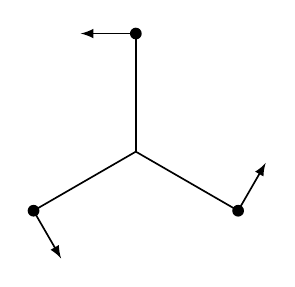
\begin{tikzpicture}
                \draw [semithick,-latex] (0,0) -- (90:1.5) node[circle,fill,inner sep=1.5pt]{} -- ++(180:0.7);
                \draw [semithick,-latex] (0,0) -- (-30:1.5) node[circle,fill,inner sep=1.5pt]{} -- ++(60:0.7);
                \draw [semithick,-latex] (0,0) -- (-150:1.5) node[circle,fill,inner sep=1.5pt]{} -- ++(-60:0.7);
            \end{tikzpicture}
            \caption{Rotational basis vectors.}
            \label{fig:rotationalBasis}
        \end{figure}
    \end{itemize}
\end{itemize}



\section{Chapter 13: Molecular Spectroscopy}
\emph{From \textcite{bib:McQuarrieSimon}.}
\begin{itemize}
    \item \marginnote{11/30:}\textbf{Spectroscopy}: The study of the interaction of electromagnetic radiation with atoms and molecules.
    \item "Electromagnetic radiation is customarily divided into different energy regions reflecting the different types of molecular processes that can be caused by such radiation" \parencite[495-96]{bib:McQuarrieSimon}.
    \item Vibrational selection rule: Transitions among vibrational levels resulting from the absorption of radiation have $\Delta v=\pm 1$ and have a dipole moment that varies during the vibration.
    \begin{itemize}
        \item For a harmonic oscillator, the spectrum consists of one line in the infrared region at the frequency $\nu_\text{obs}=\sqrt{k/\mu}/2\pi$.
    \end{itemize}
    \item \textbf{Vibrational term}: The vibrational energy of a molecule. \emph{Denoted by} $\bm{G(v)}$. \emph{Units} $\si{\per\centi\meter}$. \emph{Given by}
    \begin{equation*}
        G(v) = \frac{E_v}{hc}
    \end{equation*}
    where $E_v=(v+1/2)h\nu$ and $\nu=\sqrt{k/\mu}/2\pi$.
    \item Each energy $E_J=\hbar^2/(2I)\cdot J(J+1)$ of the rigid rotator is associated with degeneracy $g_J=2J+1$.
\end{itemize}




\end{document}